% !TEX root = ../../main.tex
\section{Artifical data generation}\label{sec:artificial_data_generation}
In this section we present four data sets as used by \cite{camci2010change,takeuchi2006unifying} to provide for a objetive performance comparison.
All the data sets are modeled by a second-order \gls{ar}-model as in \Cref{eq:artificial_data_sets_model}, where $\epsilon_t$ is a Gaussian distribution modeling the noise with mean $0$ and variance $\sigma^2 = 1$, $a_1 = 0.6$ and $a_2 = -0.5$.
\begin{equation}\label{eq:artificial_data_sets_model}
  x_t = a_1 x_{t-1} + a_2 x_{t-2} + \epsilon_t,
\end{equation}
The length of $x_t$ is $10000$ and change points are generated at each $y \times 10000^\text{th}$ data point, with $y = (1, 2, 3, \dots 9)$.

Using this general \gls{ar}-model, we create four different data sets.
Each data set is characterized by a change in mean, variance, or both of the Gaussian term $\epsilon_t$:
\begin{enumerate}
  \item \textbf{Fixed increasing mean:} at each change point $y$ the mean is increased with $\Delta(y) = 5$.
  This set origins as the first data set of Camci~\cite{camci2010change}.
  See \Cref{fig:camci_fixed_increasing_mean,fig:camci_fixed_increasing_mean_thresholds}.

  \item \textbf{Reduced increasing mean:} at each change point $y$ the mean is increased with $\Delta(y) = 10 - y$.
  This set origins as the first data set of Takeuchi \etal \cite{takeuchi2006unifying}.
  See \Cref{fig:takeuchi_reduced_increasing_mean,fig:takeuchi_reduced_increasing_mean_thresholds}.

  \item \textbf{Reduced increasing mean, increasing variance:} at each change point $y$ the mean is increased with $\Delta(y) = 10 - y$ and the standard deviation is of $\epsilon_t$ is $0.1 / (0.01 + (10000 - x)/1000)$.
  This set origins as the second set of Camci~\cite{camci2010change}.
  See \Cref{fig:camci_reduced_increasing_mean_increasing_variance,fig:camci_reduced_increasing_mean_increasing_variance_thresholds}

  \item \textbf{Alternating variance:} at each change point $y$ the variance $\sigma^2$ is set to $9.0$ when $y$ is odd, and to $1.0$ otherwise.
  This set origins as the thirds sets from Camci~\cite{camci2010change} and Takeuchi \etal \cite{takeuchi2006unifying}.
  See \Cref{fig:camci_takeuchi_alternating_variance,fig:camci_takeuchi_alternating_variance_thresholds}.
\end{enumerate}

% =====

\begin{figure}
\centering
  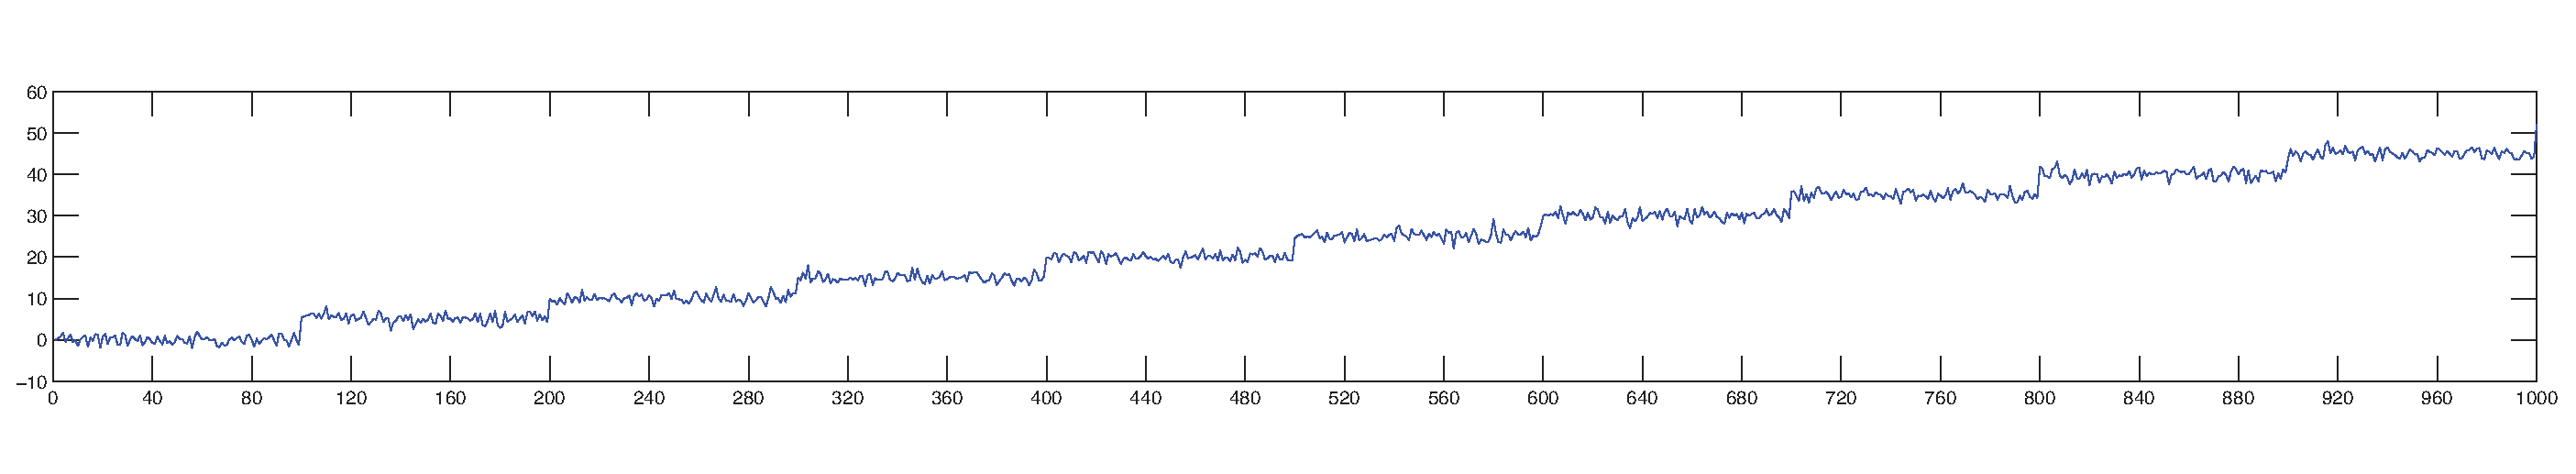
\includegraphics[width=1\textwidth]{./Figures/chapter5/camci_fixed_increasing_mean.eps}
  \caption[Fixed increasing mean]{Fixed increasing mean}
  \label{fig:camci_fixed_increasing_mean}
\end{figure}

\begin{figure}
\centering
  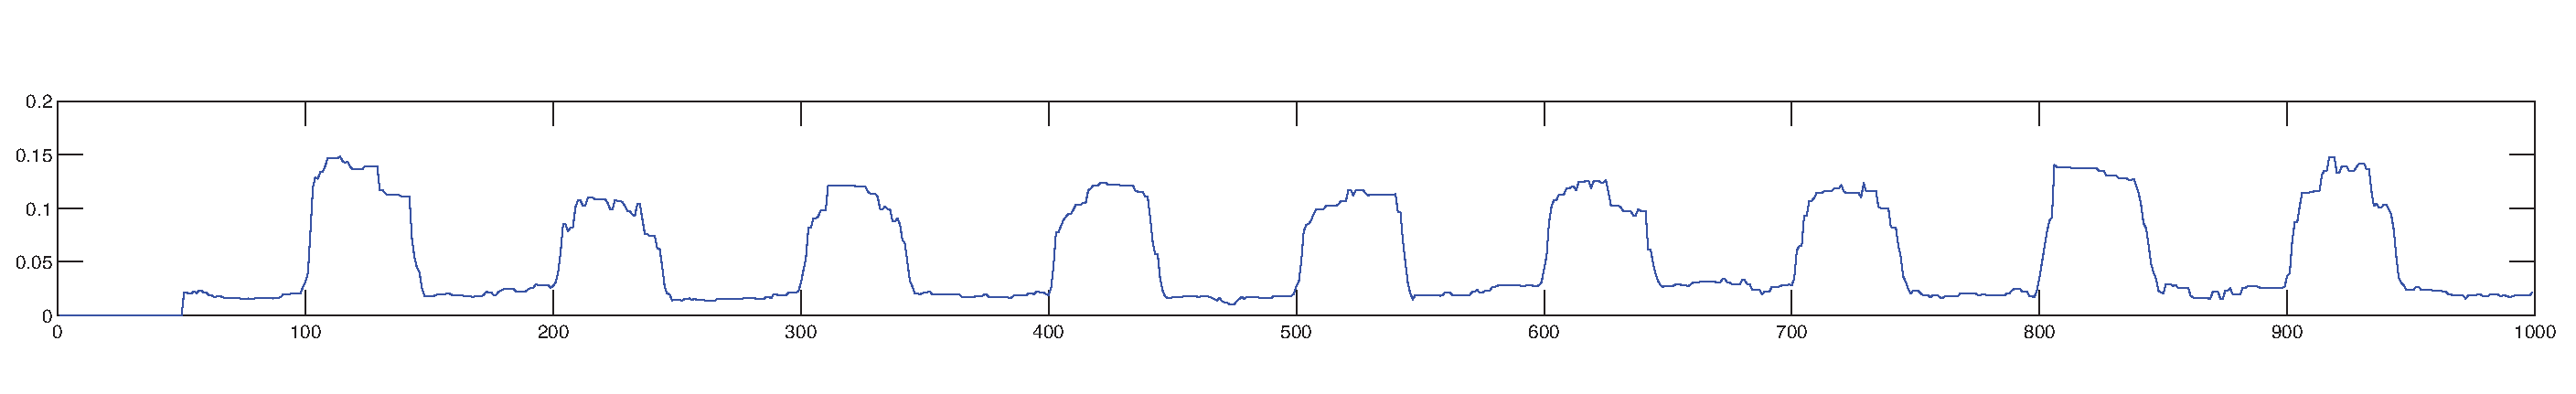
\includegraphics[width=1\textwidth]{./Figures/chapter5/camci_fixed_increasing_mean_thresholds.eps}
  \caption[Fixed increasing mean, thresholds]{Fixed increasing mean, thresholds}
  \label{fig:camci_fixed_increasing_mean_thresholds}
\end{figure}

% =====

\begin{figure}
\centering
  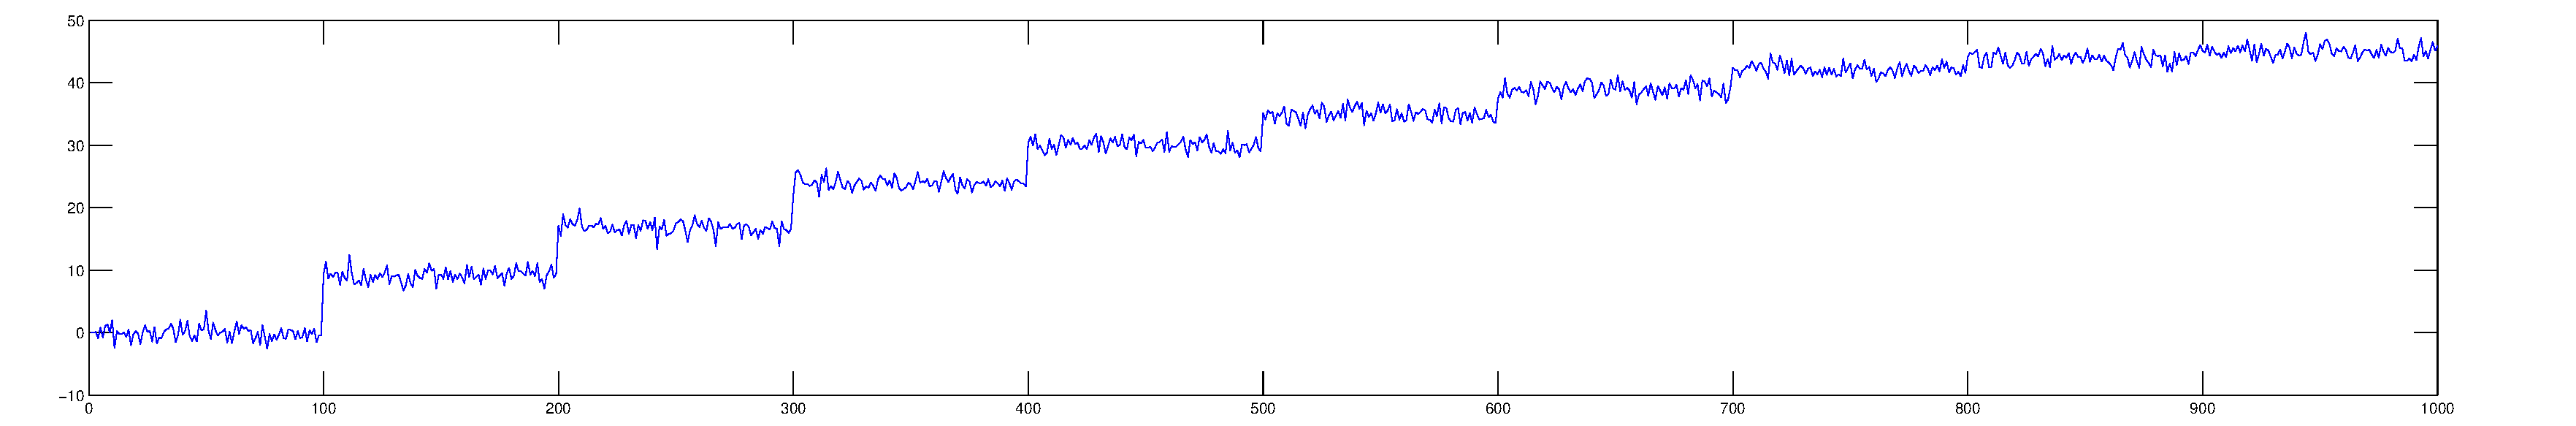
\includegraphics[width=1\textwidth]{./Figures/chapter5/takeuchi_reduced_increasing_mean.eps}
  \caption[Reduced increasing mean]{Reduced increasing mean}
  \label{fig:takeuchi_reduced_increasing_mean}
\end{figure}

\begin{figure}
\centering
  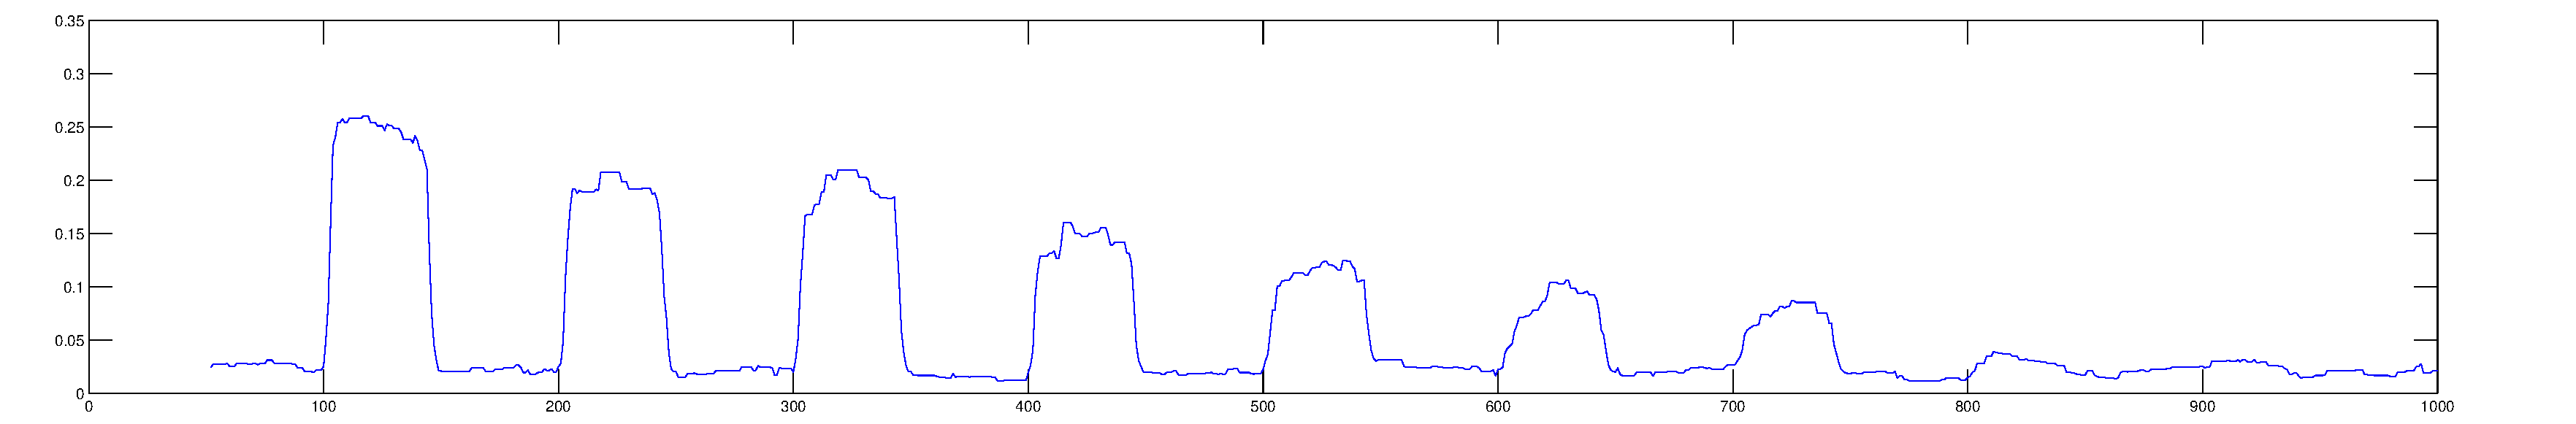
\includegraphics[width=1\textwidth]{./Figures/chapter5/takeuchi_reduced_increasing_mean_thresholds.eps}
  \caption[Reduced increasing mean, thresholds]{Reduced increasing mean, thresholds}
  \label{fig:takeuchi_reduced_increasing_mean_thresholds}
\end{figure}

% =====

\begin{figure}
\centering
  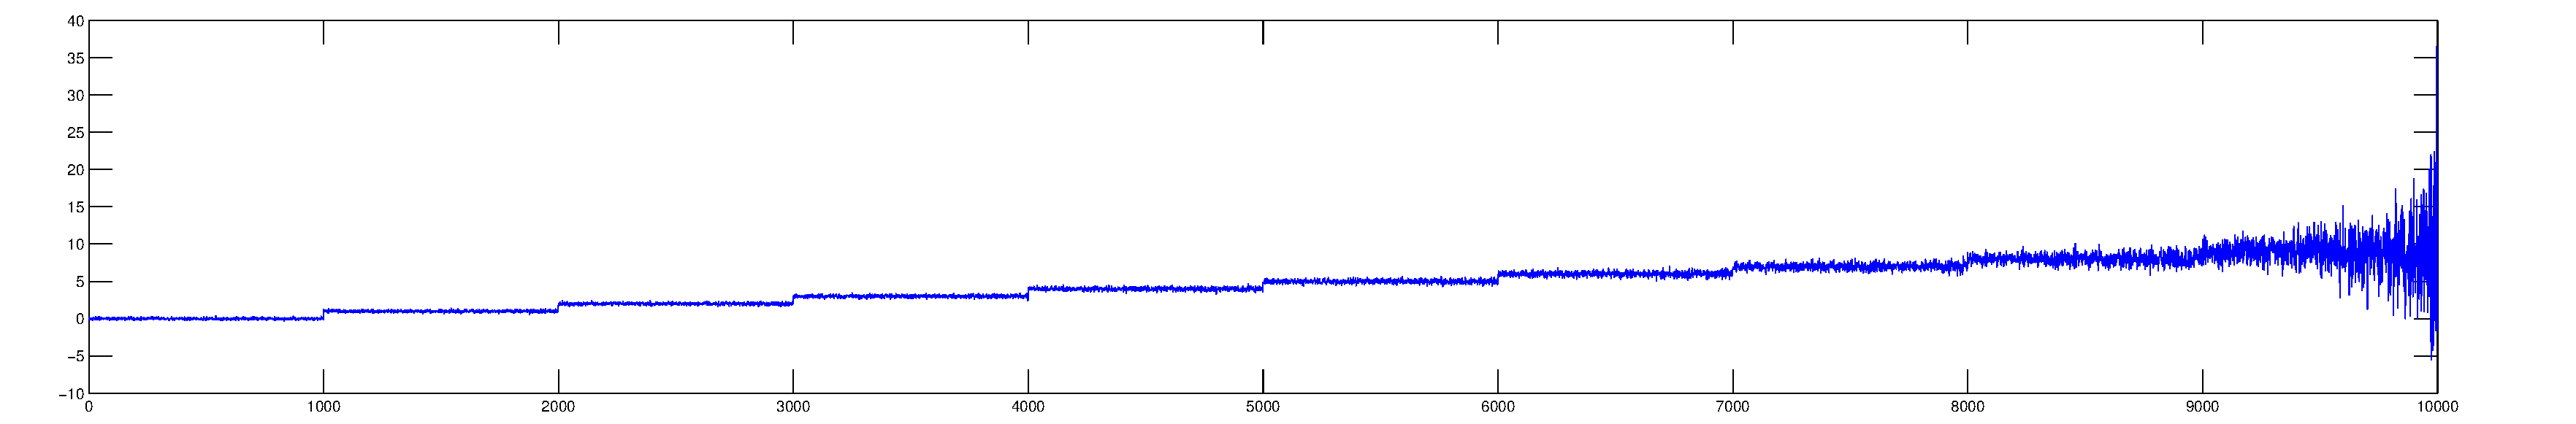
\includegraphics[width=1\textwidth]{./Figures/chapter5/camci_reduced_increasing_mean_increasing_variance.eps}
  \caption[Reduced increasing mean, increasing variance]{Reduced increasing mean, increasing variance.}
  \label{fig:camci_reduced_increasing_mean_increasing_variance}
\end{figure}

\begin{figure}
\centering
  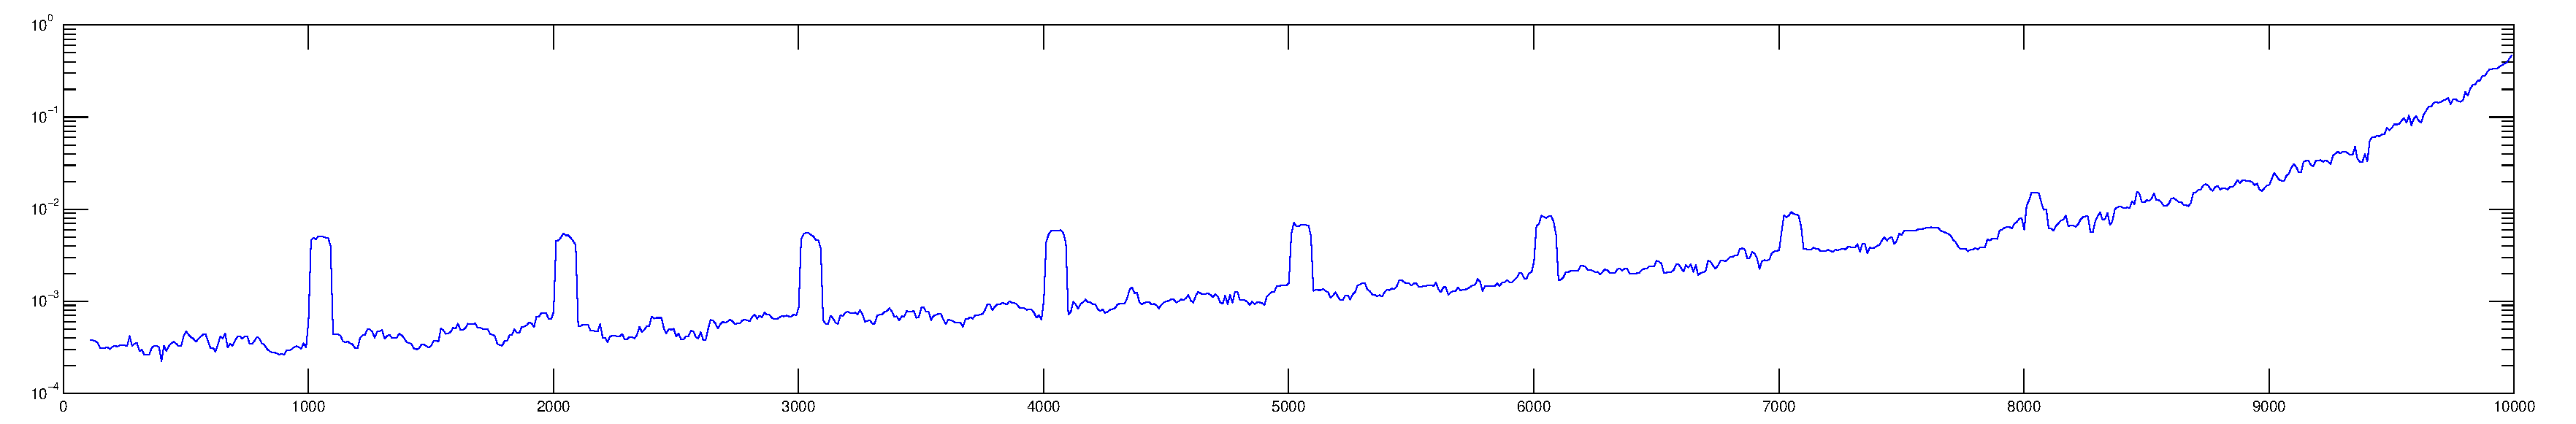
\includegraphics[width=1\textwidth]{./Figures/chapter5/camci_reduced_increasing_mean_increasing_variance_thresholds.eps}
  \caption[Reduced increasing mean, increasing variance, thresholds]{Reduced increasing mean, increasing variance, thresholds (log scale)}
  \label{fig:camci_reduced_increasing_mean_increasing_variance_thresholds}
\end{figure}

% =====

\begin{figure}
\centering
  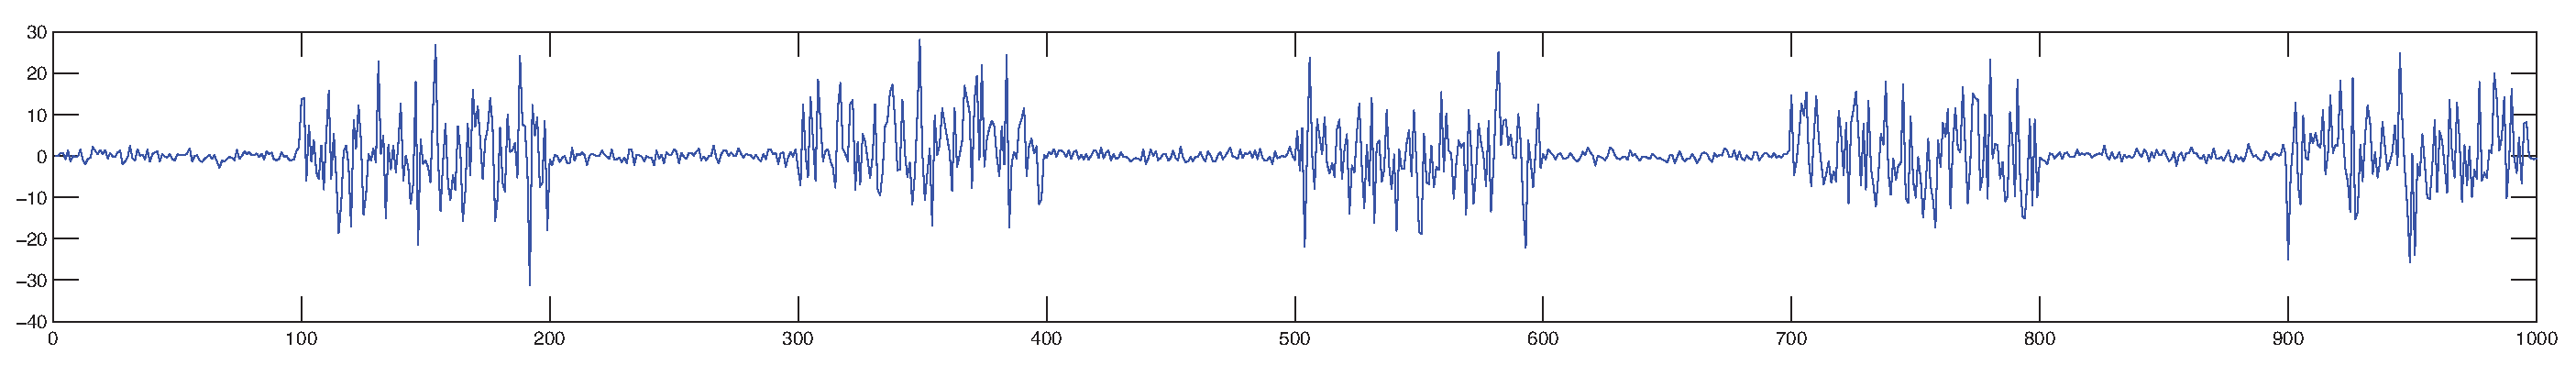
\includegraphics[width=1\textwidth]{./Figures/chapter5/camci_takeuchi_alternating_variance.eps}
  \caption[Alternating variance]{Alternating variance}
  \label{fig:camci_takeuchi_alternating_variance}
\end{figure}

\begin{figure}
\centering
  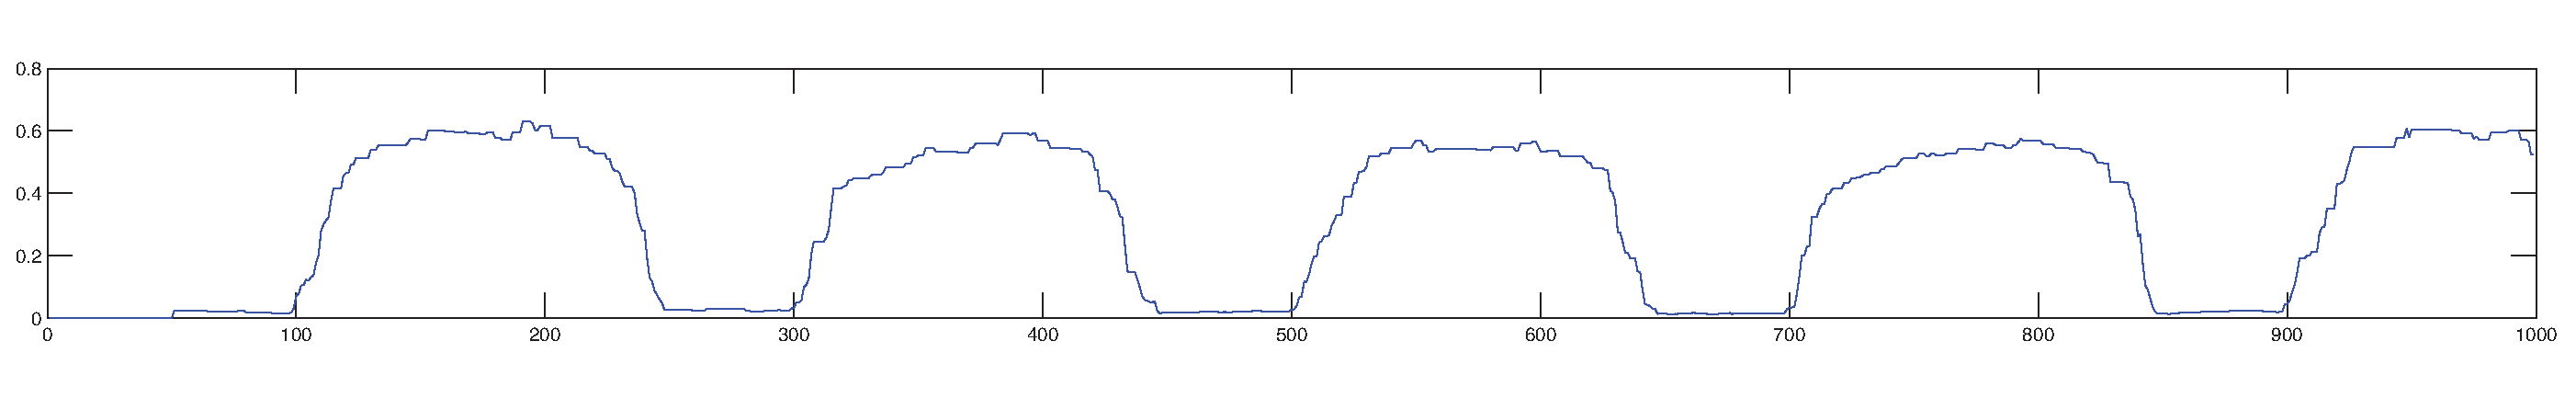
\includegraphics[width=1\textwidth]{./Figures/chapter5/camci_takeuchi_alternating_variance_thresholds.eps}
  \caption[Alternating variance, thresholds]{Alternating variance, thresholds}
  \label{fig:camci_takeuchi_alternating_variance_thresholds}
\end{figure}